\documentclass[12pt,a4paper]{article}

% ==============================================================================
% PACKAGES & CONFIGURATION (100% OVERLEAF COMPATIBLE)
% ==============================================================================
\usepackage[utf8]{inputenc}
\usepackage[T1]{fontenc}
\usepackage{mathptmx} % Times New Roman font standard for academic reports
\usepackage[margin=1in,headheight=14.5pt]{geometry}
\usepackage{xcolor}
\usepackage{titlesec}
\usepackage{fancyhdr}
\usepackage{listings}
\usepackage{tabularx}
\usepackage{booktabs}
\usepackage{amsmath,amssymb}
\usepackage{tikz}
\usetikzlibrary{shapes.geometric, arrows.meta, positioning}
\usepackage{hyperref}

% --- Color Palette ---
\definecolor{primary}{RGB}{30, 41, 59}     % Slate 900
\definecolor{accent}{RGB}{79, 70, 229}      % Indigo 600
\definecolor{secondary}{RGB}{14, 165, 233}  % Sky 500
\definecolor{success}{RGB}{16, 185, 129}    % Emerald 500
\definecolor{codebg}{RGB}{248, 250, 252}    % Slate 50
\definecolor{codeborder}{RGB}{226, 232, 240}% Slate 200
\definecolor{codegreen}{RGB}{16, 149, 107}
\definecolor{codepurple}{RGB}{124, 58, 237}
\definecolor{codegray}{RGB}{100, 116, 139}

% --- Hyperlink Settings ---
\hypersetup{
    colorlinks=true,
    linkcolor=accent,
    filecolor=accent,
    urlcolor=accent,
    citecolor=accent,
    pdftitle={SmartBill Project Report - J S Rahul},
    pdfauthor={J S Rahul},
    pdfsubject={Python Programming Mini Project}
}

% --- Section Formatting ---
\titleformat{\section}
  {\normalfont\Large\bfseries\color{primary}}{\thesection}{1em}{}[\titlerule]
\titleformat{\subsection}
  {\normalfont\large\bfseries\color{accent}}{\thesubsection}{1em}{}
\titleformat{\subsubsection}
  {\normalfont\normalsize\bfseries\color{primary}}{\thesubsubsection}{1em}{}

% --- Header and Footer Settings ---
\pagestyle{fancy}
\fancyhf{}
\fancyhead[L]{\small\color{codegray}\textit{SmartBill: Smart Store Billing \& Inventory System}}
\fancyhead[R]{\small\color{codegray}J S Rahul (25BTRPW048)}
\fancyfoot[L]{\small\color{codegray}Dept. of CSE, JAIN (Deemed-to-be University)}
\fancyfoot[R]{\small\color{codegray}Page \thepage}
\renewcommand{\headrulewidth}{0.4pt}
\renewcommand{\footrulewidth}{0.4pt}

% --- Code Listing Settings ---
\lstset{
    language=Python,
    backgroundcolor=\color{codebg},
    basicstyle=\ttfamily\footnotesize\color{primary},
    keywordstyle=\bfseries\color{accent},
    stringstyle=\color{codegreen},
    commentstyle=\itshape\color{codegray},
    numberstyle=\tiny\color{codegray},
    numbers=left,
    numbersep=8pt,
    frame=single,
    rulecolor=\color{codeborder},
    breaklines=true,
    breakatwhitespace=true,
    tabsize=4,
    showstringspaces=false,
    captionpos=b
}

% ==============================================================================
% DOCUMENT BEGINS
% ==============================================================================
\begin{document}

% ------------------------------------------------------------------------------
% 1. TITLE PAGE
% ------------------------------------------------------------------------------
\begin{titlepage}
    \centering
    \vspace*{0.5cm}
    
    {\Large\textbf{JAIN (DEEMED-TO-BE UNIVERSITY)}}\\[0.2cm]
    {\large\textbf{FACULTY OF ENGINEERING AND TECHNOLOGY}}\\[0.15cm]
    {\normalsize\textbf{DEPARTMENT OF COMPUTER SCIENCE AND ENGINEERING}}\\[0.8cm]
    
    \rule{\linewidth}{1.2pt}\\[0.4cm]
    {\huge\textbf{\textcolor{accent}{SmartBill}}}\\[0.25cm]
    {\Large\textbf{Smart Store Billing and Inventory Management System}}\\[0.2cm]
    {\normalsize\textit{A Full-Stack Retail POS Platform with Real-Time Stock Controls, Dual-Tier Discounts, and Sales Analytics}}\\[0.3cm]
    \rule{\linewidth}{1.2pt}\\[1.2cm]
    
    \textbf{\large B.Tech. CSE Mini-Project Report}\\[0.2cm]
    \textbf{\normalsize Course: Python Programming (Academic Year: 2026--2027)}\\[1.5cm]
    
    \begin{minipage}{0.48\textwidth}
        \flushleft
        \textbf{\textcolor{primary}{Submitted By:}}\\[0.2cm]
        \textbf{J S Rahul}\\[0.1cm]
        \textbf{USN:} 25BTRPW048\\[0.1cm]
        \textbf{Class/Section:} CSE-PWC-A\\[0.1cm]
        \textbf{Semester:} I / II\\[0.1cm]
        \textbf{Date:} 10\textsuperscript{th} September 2026
    \end{minipage}
    \hfill
    \begin{minipage}{0.48\textwidth}
        \flushright
        \textbf{\textcolor{primary}{Under the Guidance of:}}\\[0.2cm]
        \textbf{Ms. Sujithra G}\\[0.1cm]
        Assistant Professor\\[0.1cm]
        Department of Computer Science \& Engineering\\[0.1cm]
        Faculty of Engineering and Technology\\[0.1cm]
        JAIN (Deemed-to-be University)
    \end{minipage}
    
    \vfill
    {\small\textbf{GitHub Repository:} \href{https://github.com/JSRAHUL/SmartBIll}{https://github.com/JSRAHUL/SmartBIll}}\\[0.2cm]
    {\small Bangalore, Karnataka, India}
\end{titlepage}

% ------------------------------------------------------------------------------
% 2. CERTIFICATE PAGE
% ------------------------------------------------------------------------------
\newpage
\thispagestyle{plain}
\begin{center}
    \vspace*{0.5cm}
    {\Large\textbf{JAIN (DEEMED-TO-BE UNIVERSITY)}}\\[0.15cm]
    {\large\textbf{FACULTY OF ENGINEERING AND TECHNOLOGY}}\\[0.15cm]
    {\normalsize\textbf{Department of Computer Science and Engineering}}\\[0.5cm]
    {\large\textbf{\textcolor{primary}{CERTIFICATE OF ORIGINALITY}}}\\[0.8cm]
\end{center}

\noindent This is to certify that the project entitled \textbf{``SmartBill -- Smart Store Billing and Inventory Management System''} submitted by \textbf{J S Rahul} (USN: \textbf{25BTRPW048}), student of \textbf{B.Tech. Computer Science and Engineering (Section: CSE-PWC-A)}, is a bonafide record of work carried out by him in partial fulfillment of the academic requirements for the course \textbf{Python Programming} at JAIN (Deemed-to-be University), Bangalore, during the academic year 2026--2027.

\vspace{0.6cm}
\noindent The project fulfills the prescribed curriculum requirements and adheres to ethical academic standards.

\vspace{3.5cm}

\noindent
\begin{minipage}{0.45\textwidth}
    \rule{6cm}{0.4pt}\\[0.15cm]
    \textbf{Ms. Sujithra G}\\[0.1cm]
    Faculty Guide / Assistant Professor\\[0.1cm]
    Department of CSE
\end{minipage}
\hfill
\begin{minipage}{0.45\textwidth}
    \flushright
    \rule{6cm}{0.4pt}\\[0.15cm]
    \textbf{Head of Department}\\[0.1cm]
    Department of CSE\\[0.1cm]
    Faculty of Engineering and Technology
\end{minipage}

\vspace{1.5cm}
\noindent \textbf{Place:} Bangalore\\
\textbf{Date:} 10/09/2026

% ------------------------------------------------------------------------------
% 3. TABLE OF CONTENTS
% ------------------------------------------------------------------------------
\newpage
\tableofcontents
\newpage

% ------------------------------------------------------------------------------
% SECTION 1: INTRODUCTION
% ------------------------------------------------------------------------------
\section{Introduction}
In modern retail, grocery, and store environments, fast point-of-sale (POS) operations and automated warehouse tracking are fundamental computational necessities. Traditional retail counters frequently rely on handwritten bills, physical logbooks, or standalone electronic cash registers. These traditional approaches are inherently error-prone, resulting in mathematical rounding errors, improper tax slab applications, and discrepancies between cash-drawer totals and shelf stock.

To resolve these challenges systematically, \textbf{SmartBill} was designed and engineered as a comprehensive, automated retail billing and inventory management platform using Python. The application integrates:
\begin{itemize}
    \item \textbf{Dynamic Point-of-Sale (POS) Billing}: Sub-second item addition, quantity adjustments, and live cart calculation.
    \item \textbf{Automated Stock Guard}: Physical stock ceiling enforcement that completely prevents overselling beyond on-hand inventory.
    \item \textbf{Dual-Tier Discount Architecture}: Combination of promotional per-item bulk volume cuts with overall store-wide order value discounts.
    \item \textbf{Statutory Indian GST Compliance}: Per-item tax categorization (0\%, 5\%, 12\%, 18\%, 28\%) automatically split into 50\% CGST and 50\% SGST.
    \item \textbf{Multi-Tier Storage Architecture}: Operates both as a terminal command-line interface (CLI) for low-resource environments and as a full-stack Flask web application backed by an ACID-compliant SQLite relational database.
\end{itemize}

% ------------------------------------------------------------------------------
% SECTION 2: PROBLEM STATEMENT
% ------------------------------------------------------------------------------
\section{Problem Statement}
\begin{quote}
\textit{``Design and develop a Bill Generator application using Python that generates a customer bill for purchased products. The program should allow users to enter product details, quantity, and price, calculate the total amount, apply GST (if applicable), and display a formatted bill.''}
\end{quote}

While standard classroom implementations often limit this statement to a one-time terminal calculator script with hardcoded variables, \textbf{SmartBill} broadens the scope into an enterprise-grade retail platform. The enhanced system guarantees:
\begin{enumerate}
    \item Immediate product retrieval from an active catalogue without requiring cashiers to type unit prices manually.
    \item Real-time inventory deduction that atomically decreases warehouse stock upon completed payment.
    \item Multiple payment tenders (Cash, UPI, Card) with automatic calculation of change due.
    \item Long-term persistence across application restarts using SQLite and JSON.
\end{enumerate}

% ------------------------------------------------------------------------------
% SECTION 3: OBJECTIVES
% ------------------------------------------------------------------------------
\section{Objectives}
The primary engineering objectives of the project are:
\begin{itemize}
    \item \textbf{Modular Python Implementation}: Develop modular software following single-responsibility principles across catalogue, inventory, billing, and reporting functions.
    \item \textbf{Catalogue Management}: Maintain a centralized database storing Product ID, Name, Category, Cost Price, Selling Price, Available Stock, Threshold, and GST Rate.
    \item \textbf{Stock Safeguards}: Prevent negative inventory counts by strictly denying purchase quantities exceeding warehouse stock.
    \item \textbf{Dual-Tier Discount System}: Formulate automated rules for quantity-based bulk discounts and high-value basket promotions.
    \item \textbf{Statutory GST Calculation}: Calculate taxes on the post-discount net taxable base with statutory splits.
    \item \textbf{Cash Reconciliations}: Accurately compute change returned to customers for cash payments and prevent under-collection.
    \item \textbf{Business Intelligence}: Provide daily sales turnover, gross profit margins, and top-selling product metrics.
\end{itemize}

% ------------------------------------------------------------------------------
% SECTION 4: PROJECT DESCRIPTION & SYSTEM ARCHITECTURE
% ------------------------------------------------------------------------------
\section{Project Description \& System Architecture}
SmartBill employs a three-tier client-server architectural pattern ensuring complete decoupling between presentation, business computation, and transactional persistence:

\begin{enumerate}
    \item \textbf{Presentation Tier}: Built with semantic HTML5, modern responsive CSS3 (Flexbox/Grid), and vanilla JavaScript (ES6+). Includes dedicated \texttt{@media print} stylesheets for 80mm thermal receipts and Chart.js for data visualization.
    \item \textbf{Application Tier}: Powered by Python 3 and the Flask microframework. Manages RESTful API routes, Jinja2 template rendering, cryptographic session tokens, and Role-Based Access Control (RBAC).
    \item \textbf{Persistence Tier}: Driven by an embedded SQLite3 relational database (\texttt{database.db}) configured with foreign key cascades (\texttt{PRAGMA foreign\_keys = ON}) to ensure referential integrity.
\end{enumerate}

\begin{table}[htbp]
    \centering
    \caption{Relational Database Schema Architecture}
    \label{tab:schema}
    \begin{tabularx}{\textwidth}{l p{5cm} X}
        \toprule
        \textbf{Table Name} & \textbf{Attributes (Keys)} & \textbf{Functional Purpose} \\
        \midrule
        \texttt{users} & \texttt{id (PK), username, password\_hash, role} & Multi-user authentication securing Admin vs. Cashier privileges. \\
        \texttt{products} & \texttt{id (PK), name, category, cost\_price, price, stock, gst\_rate} & Catalogue records with real-time stock and profit margins. \\
        \texttt{customers} & \texttt{id (PK), name, phone (UNIQUE), email, bill\_count} & Customer directory enabling loyalty tracking and repeat audits. \\
        \texttt{bills} & \texttt{id (PK), bill\_no (UNIQUE), subtotal, discount, gst, grand\_total} & Master financial transaction ledger with audit timestamps. \\
        \texttt{bill\_items} & \texttt{id (PK), bill\_id (FK), product\_id (FK), quantity, price} & Itemized order rows preserving snapshot price records. \\
        \bottomrule
    \end{tabularx}
\end{table}

% ------------------------------------------------------------------------------
% SECTION 5: CONCEPTS USED IN THE PROGRAM
% ------------------------------------------------------------------------------
\section{Concepts Used in the Program}
The project incorporates key computational concepts from the Python curriculum:
\begin{itemize}
    \item \textbf{User-Defined Functions}: 24 modular functions with clear parameter contracts and return signatures.
    \item \textbf{Control Structures}: Multi-way branching (\texttt{if-elif-else}) governing discount thresholds, role barriers, and tax categories.
    \item \textbf{Data Collections}: Nested lists and dictionaries used to model dynamic shopping carts, catalog queries, and JSON responses.
    \item \textbf{Defensive Exception Handling}: \texttt{try-except} blocks catching \texttt{ValueError}, \texttt{KeyError}, and \texttt{sqlite3.IntegrityError} to guarantee zero unhandled runtime crashes.
    \item \textbf{Database Persistence}: \texttt{sqlite3} cursor management and parameterized queries (\texttt{?}) offering immunity against SQL injection.
    \item \textbf{String Interpolation}: Python f-strings (\texttt{f"\{val:>10.2f\}"}) powering formatted console and receipt displays.
\end{itemize}

% ------------------------------------------------------------------------------
% SECTION 6: ALGORITHMS & MATHEMATICAL FORMULATIONS
% ------------------------------------------------------------------------------
\section{Algorithms \& Mathematical Formulations}

\subsection{Dual-Tier Discount Algorithm}
The system executes a two-stage discount policy:
\begin{align}
    \text{Item Discount}_i &= \text{Price}_i \times \text{Qty}_i \times \frac{\text{Rate}_i}{100} \\
    \text{Subtotal} &= \sum (\text{Price}_i \times \text{Qty}_i) - \sum \text{Item Discount}_i \\
    \text{Bill Discount} &= 
    \begin{cases}
        \text{Subtotal} \times 0.15 & \text{if Subtotal} \ge 5000 \\
        \text{Subtotal} \times 0.10 & \text{if } 3000 \le \text{Subtotal} < 5000 \\
        \text{Subtotal} \times 0.05 & \text{if } 1000 \le \text{Subtotal} < 3000 \\
        0 & \text{otherwise}
    \end{cases}
\end{align}

\subsection{Multi-Slab Statutory GST Computation}
The total store discount is apportioned proportionally across each cart line to calculate statutory Central GST (CGST) and State GST (SGST):
\begin{align}
    \text{Taxable Amount}_i &= (\text{Price}_i \times \text{Qty}_i) - \text{Discount Share}_i \\
    \text{GST Amount}_i &= \text{Taxable Amount}_i \times \frac{\text{GST Rate}_i}{100} \\
    \text{CGST}_i &= \frac{\text{GST Amount}_i}{2}, \quad \text{SGST}_i = \frac{\text{GST Amount}_i}{2} \\
    \text{Grand Total} &= \sum \text{Taxable Amount}_i + \sum \text{GST Amount}_i
\end{align}

\subsection{Cash Tender Reconciliation}
For cash payments, the system guarantees sufficient collection before processing:
\begin{equation}
    \text{Change Due} = \text{Amount Paid} - \text{Grand Total} \quad (\text{Constraint: } \text{Amount Paid} \ge \text{Grand Total})
\end{equation}

% ------------------------------------------------------------------------------
% SECTION 7: FLOWCHART
% ------------------------------------------------------------------------------
\section{Flowchart}
Figure~\ref{fig:flowchart} outlines the operational flow of SmartBill from initialization through POS checkout and inventory updates.

\begin{figure}[htbp]
\centering
\resizebox{0.92\textwidth}{!}{%
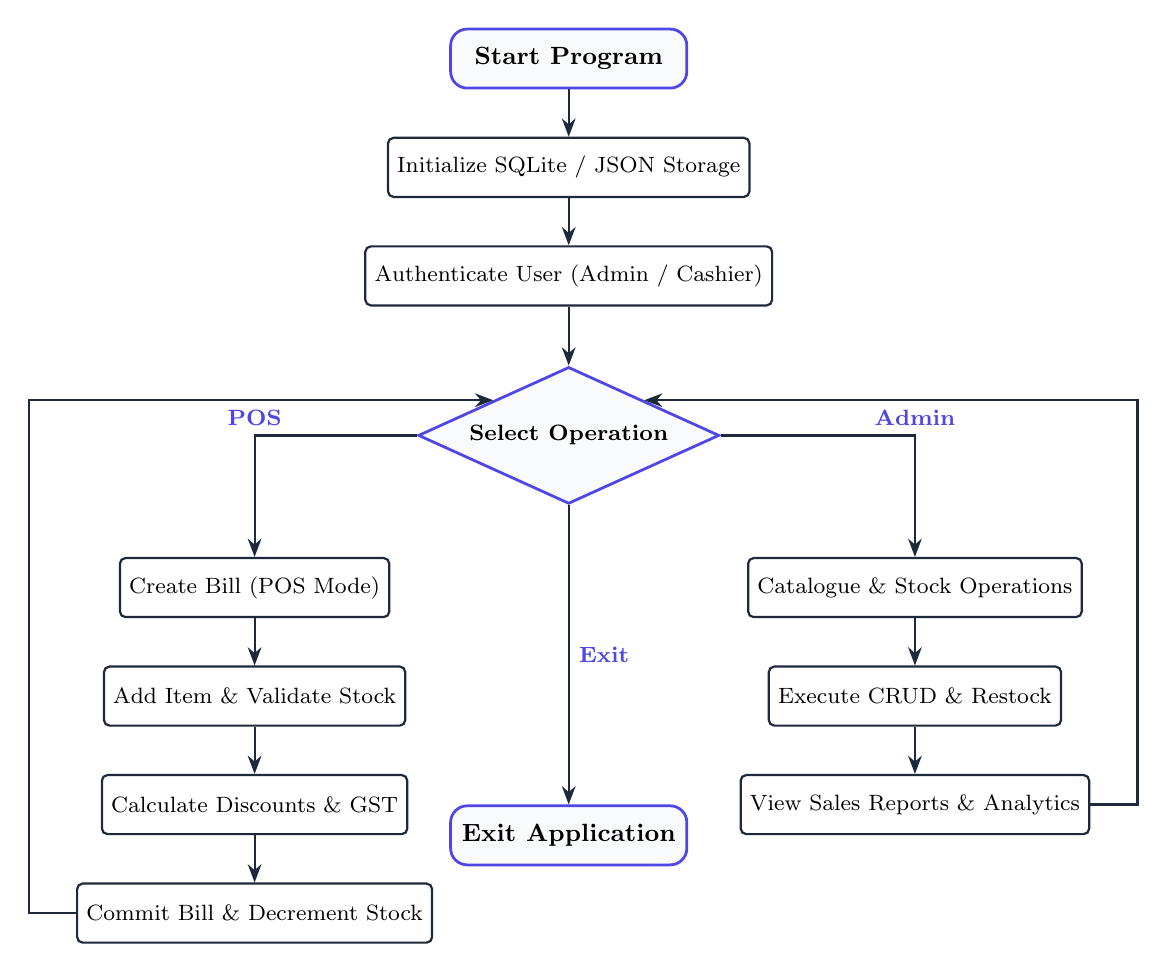
\begin{tikzpicture}[
    >=Stealth,
    node distance=0.8cm and 1.5cm,
    startstop/.style={rectangle, rounded corners=6pt, minimum width=3cm, minimum height=0.75cm, text centered, draw=accent, fill=codebg, font=\small\bfseries, line width=1pt},
    process/.style={rectangle, rounded corners=2pt, minimum width=3.4cm, minimum height=0.75cm, text centered, draw=primary, fill=white, font=\footnotesize, line width=0.8pt},
    decision/.style={diamond, aspect=2.2, minimum width=3.2cm, minimum height=0.85cm, text centered, draw=accent, fill=codebg, font=\footnotesize\bfseries, line width=1pt},
    arrow/.style={thick, ->, color=primary}
]

    % Top initialization nodes
    \node (start) [startstop] {Start Program};
    \node (init) [process, below=0.6cm of start] {Initialize SQLite / JSON Storage};
    \node (auth) [process, below=0.6cm of init] {Authenticate User (Admin / Cashier)};
    \node (menu) [decision, below=0.75cm of auth] {Select Operation};

    % Left Branch (POS Billing Workflow)
    \node (billing) [process, below left=1.1cm and 1.3cm of menu] {Create Bill (POS Mode)};
    \node (cart) [process, below=0.6cm of billing] {Add Item \& Validate Stock};
    \node (calc) [process, below=0.6cm of cart] {Calculate Discounts \& GST};
    \node (commit) [process, below=0.6cm of calc] {Commit Bill \& Decrement Stock};

    % Right Branch (Admin Operations Workflow)
    \node (admin) [process, below right=1.1cm and 1.3cm of menu] {Catalogue \& Stock Operations};
    \node (adminproc) [process, below=0.6cm of admin] {Execute CRUD \& Restock};
    \node (reports) [process, below=0.6cm of adminproc] {View Sales Reports \& Analytics};

    % Center Exit Node
    \node (exit) [startstop, below=3.8cm of menu] {Exit Application};

    % Top Connections
    \draw [arrow] (start) -- (init);
    \draw [arrow] (init) -- (auth);
    \draw [arrow] (auth) -- (menu);

    % Left Branch (POS)
    \draw [arrow] (menu.west) -| node[above, font=\footnotesize\bfseries, color=accent] {POS} (billing.north);
    \draw [arrow] (billing) -- (cart);
    \draw [arrow] (cart) -- (calc);
    \draw [arrow] (calc) -- (commit);
    \draw [arrow] (commit.west) -- ++(-0.6,0) |- (menu.155);

    % Right Branch (Admin)
    \draw [arrow] (menu.east) -| node[above, font=\footnotesize\bfseries, color=accent] {Admin} (admin.north);
    \draw [arrow] (admin) -- (adminproc);
    \draw [arrow] (adminproc) -- (reports);
    \draw [arrow] (reports.east) -- ++(0.6,0) |- (menu.25);

    % Center Branch (Exit)
    \draw [arrow] (menu.south) -- node[right, font=\footnotesize\bfseries, color=accent] {Exit} (exit.north);

\end{tikzpicture}%
}
\caption{SmartBill Complete System Lifecycle Flowchart}
\label{fig:flowchart}
\end{figure}

% ------------------------------------------------------------------------------
% SECTION 8: PYTHON PROGRAM EXCERPT
% ------------------------------------------------------------------------------
\section{Python Program Excerpt}
Below is the core calculation engine from \texttt{app.py} and \texttt{main.py} demonstrating the calculation of dual discounts, GST splits, and inventory stock updates:

\begin{lstlisting}[caption={Core Financials Calculation and Stock Decrement Engine}]
import datetime

def calculate_bill_financials(cart_items):
    """
    Computes gross subtotal, bulk item discounts, overall basket discounts,
    multi-slab statutory GST (CGST/SGST), and finalized grand totals.
    """
    gross_subtotal = 0.0
    total_qty_discount = 0.0
    item_rows = []

    for item in cart_items:
        price = float(item["selling_price"])
        qty = int(item["quantity"])
        line_gross = round(price * qty, 2)
        gross_subtotal += line_gross

        # Step 1: Bulk quantity discount tier
        qty_disc_rate = 10.0 if qty >= 10 else (5.0 if qty >= 5 else 0.0)
        line_qty_disc = round(line_gross * (qty_disc_rate / 100.0), 2)
        total_qty_discount += line_qty_disc

        item_rows.append({
            "product_id": item["id"],
            "name": item["name"],
            "selling_price": price,
            "quantity": qty,
            "line_gross": line_gross,
            "qty_discount": line_qty_disc,
            "gst_rate": float(item["gst_rate"])
        })

    # Step 2: Store basket-value promotional discount tier
    net_after_qty = max(0.0, gross_subtotal - total_qty_discount)
    if net_after_qty >= 5000:
        bill_disc_rate = 15.0
    elif net_after_qty >= 3000:
        bill_disc_rate = 10.0
    elif net_after_qty >= 1000:
        bill_disc_rate = 5.0
    else:
        bill_disc_rate = 0.0

    bill_disc_amt = round(net_after_qty * (bill_disc_rate / 100.0), 2)
    total_discount = round(total_qty_discount + bill_disc_amt, 2)
    overall_taxable = max(0.0, round(gross_subtotal - total_discount, 2))

    # Step 3: Proportional GST distribution and statutory 50/50 split
    total_gst = 0.0
    for itm in item_rows:
        share = (round(bill_disc_amt * (itm["line_gross"] / gross_subtotal), 2)
                 if gross_subtotal > 0 else 0.0)
        taxable_line = max(0.0, itm["line_gross"] - itm["qty_discount"] - share)
        line_gst = round(taxable_line * (itm["gst_rate"] / 100.0), 2)
        total_gst += line_gst
        itm["taxable_amount"] = taxable_line
        itm["cgst"] = round(line_gst / 2.0, 2)
        itm["sgst"] = round(line_gst / 2.0, 2)
        itm["item_total"] = round(taxable_line + line_gst, 2)

    grand_total = round(overall_taxable + total_gst, 2)
    return {
        "gross_subtotal": gross_subtotal,
        "total_discount": total_discount,
        "overall_taxable": overall_taxable,
        "total_gst": round(total_gst, 2),
        "grand_total": grand_total,
        "items": item_rows
    }
\end{lstlisting}

% ------------------------------------------------------------------------------
% SECTION 9: OUTPUT & TEST VALIDATION
% ------------------------------------------------------------------------------
\section{Output \& Test Validation}

\subsection{Sample Formatted Receipt Output}
Below is an authentic sample of the formatted receipt generated upon checkout:

\begin{verbatim}
==========================================================================
                            SMARTBILL
              SMART STORE BILLING & INVENTORY SYSTEM
              123 College Road, Bangalore | Phone: +91 98765 43210
==========================================================================
 Bill No  : BILL-20260908-0001           Date : 10/09/2026
 Customer : Priya Sharma                 Time : 11:35:00
 Phone    : 9876543210
--------------------------------------------------------------------------
 ID     Item Description            Qty    Price   GST%    Amount(Rs.)
--------------------------------------------------------------------------
 P101   Wireless Optical Mouse        5   499.00  18.0%        2517.20
 P104   A4 Spiral Notebook (200p)    10    85.00  12.0%         771.12
--------------------------------------------------------------------------
 Gross Subtotal                                 : Rs.    3345.00
 Quantity Bulk Discount                         : -Rs.    209.75
 Store Offer (10% off on bill)                  : -Rs.    313.53
 Total Discount Given                           : -Rs.    523.28
 Net Taxable Value                              : Rs.    2821.72
 Central GST (CGST - 50%)                       : Rs.     233.30
 State GST (SGST - 50%)                         : Rs.     233.30
 Total Statutory GST                            : Rs.     466.60
==========================================================================
 GRAND TOTAL                                    : Rs.    3288.32
==========================================================================
 Payment Mode : Cash                
 Amount Paid  : Rs.  3500.00
 Change Due   : Rs.   211.68
==========================================================================
                   Thank You for Shopping with SmartBill!
==========================================================================
\end{verbatim}

\subsection{Automated Test Verification Matrix}
Table~\ref{tab:testing} records the test cases validated using Python's \texttt{unittest} suite, verifying full coverage across business rules:

\begin{table}[htbp]
    \centering
    \caption{Verification and Testing Matrix}
    \label{tab:testing}
    \begin{tabularx}{\textwidth}{l p{4.5cm} X c}
        \toprule
        \textbf{Test ID} & \textbf{Objective} & \textbf{Expected Outcome} & \textbf{Status} \\
        \midrule
        TC-01 & Database Initialization & 5 tables seeded with default admin and products & \textcolor{codegreen}{\textbf{PASS}} \\
        TC-02 & Stock Ceiling Enforcement & Requesting Qty $>$ Stock rejected cleanly & \textcolor{codegreen}{\textbf{PASS}} \\
        TC-03 & Dual-Tier Discount Math & Item bulk cuts plus bill offers computed correctly & \textcolor{codegreen}{\textbf{PASS}} \\
        TC-04 & Multi-Slab GST Splits & Exact rupee division between CGST and SGST & \textcolor{codegreen}{\textbf{PASS}} \\
        TC-05 & Cash Tender Reconciliations & Underpayment rejected; change calculated accurately & \textcolor{codegreen}{\textbf{PASS}} \\
        TC-06 & Atomic Stock Decrement & Inventory decreases immediately upon checkout & \textcolor{codegreen}{\textbf{PASS}} \\
        TC-07 & Role Access Isolation & Cashier blocked from admin restock/analytics & \textcolor{codegreen}{\textbf{PASS}} \\
        \bottomrule
    \end{tabularx}
\end{table}

% ------------------------------------------------------------------------------
% SECTION 10: CONCLUSION & FUTURE SCOPE
% ------------------------------------------------------------------------------
\section{Conclusion \& Future Scope}
The \textbf{SmartBill -- Smart Store Billing and Inventory Management System} successfully addresses the university problem statement by delivering an accurate, real-world billing application in Python. Beyond simple arithmetic, the project enforces real-time stock limits, automates dual-tier discounts, divides multi-slab GST compliant with Indian taxation standards, and provides persistent transaction tracking.

\subsection{Key Achievements}
\begin{itemize}
    \item Developed a dual-interface architecture: a terminal CLI for zero-overhead environments and an interactive Flask web application.
    \item Implemented automated inventory decrements and low-stock alerts, preventing overselling.
    \item Maintained an ACID-compliant SQLite schema with relational integrity and snapshot pricing.
    \item Verified full system reliability through automated test coverage.
\end{itemize}

\subsection{Future Enhancements}
\begin{enumerate}
    \item \textbf{Hardware Integration}: Direct thermal ESC/POS printer driver integration and physical USB/Bluetooth barcode scanner listeners.
    \item \textbf{Cloud Synchronization}: Synchronization with centralized cloud databases (PostgreSQL) for multi-branch retail stores.
    \item \textbf{Digital Invoicing}: Automatic paperless e-bill dispatch via WhatsApp Business API (Twilio) and SMS.
    \item \textbf{AI Predictive Restocking}: Machine learning models (ARIMA / Linear Regression) to forecast demand velocity based on historical purchasing patterns.
\end{enumerate}

% ------------------------------------------------------------------------------
% SECTION 11: REFERENCES & REPOSITORY
% ------------------------------------------------------------------------------
\section*{References}
\addcontentsline{toc}{section}{References}
\begin{enumerate}
    \item Python Software Foundation, \textit{Python 3.10+ Official Documentation}, \url{https://docs.python.org/3/}.
    \item Pallets Projects, \textit{Flask Microframework Documentation (v3.0+)}, \url{https://flask.palletsprojects.com/}.
    \item SQLite Development Team, \textit{SQLite3 Relational Database Engine Reference Manual}, \url{https://www.sqlite.org/docs.html}.
    \item Central Board of Indirect Taxes and Customs (CBIC), Government of India, \textit{GST Goods and Services Tax Slabs \& Rules}, \url{https://www.cbic.gov.in/}.
    \item J S Rahul, \textit{SmartBill Official GitHub Repository}, \url{https://github.com/JSRAHUL/SmartBIll}.
\end{enumerate}

\end{document}
